% Provenance (never printed): old premiere S material on the history of plate
% tectonics (from continental drift to seafloor spreading: the ridges, the
% magnetic stripes, the ages of the drilled floor); see
% sources/book2/PROVENANCE.md. Profiles are computed in
% figdata/grade-11/magnetic_stripes.py, the age map in seafloor_age.py, the
% drilling fit in sediment_ages.py.
\chapter{महाद्वीपीय विस्थापन से समुद्री तल प्रसरण तक}\label{ch:g11:drift-to-spreading}

1950 के दशक के आरंभ में, कोलंबिया विश्वविद्यालय की लैमॉन्ट प्रयोगशाला में, मैरी थार्प नाम की
एक युवा भूवैज्ञानिक संख्याओं की लंबी पंक्तियों के सामने बैठी थीं। हर संख्या उत्तरी
अटलांटिक की एक गहराई थी, जिसे किसी जहाज़ के प्रतिध्वनि-गहराईमापी ने जहाज़ के मार्ग पर एक के बाद
एक मापा था। उन्हें एक-एक करके आलेखित करते हुए उन्होंने महासागर पार कर चुके जहाज़ों के मार्गों
के अनुदिश महासागर की तली का आकार बनाया। महासागर के बीच में तली ऊपर उठकर
एक पर्वत-श्रेणी बन जाती थी --- और हर मार्ग पर, श्रेणी के शिखर के अनुदिश,
तली फिर एक गहरी दरार में गिर जाती थी, मानो पर्वतों को बीच से
चीर दिया गया हो। यह अध्याय दिखाता है कि महासागर की तली के ऐसे मापनों ने
एक ठुकराए गए विचार, महाद्वीपों के विस्थापन, को एक सिद्धांत में कैसे बदला: महासागर की तली
कटकों पर बनती है और उनसे दूर फैलती है, और वह अपनी चट्टानों में
अपनी आयु का अभिलेख लिए चलती है।
% ledger: aip:tharp, aip:featureless, usgs:echo-sounding

\begin{recall}
महाद्वीपीय विस्थापन यह विचार है कि महाद्वीप चलते हैं; अल्फ़्रेड वेगनर ने
1912 से तटों के मेल, जीवाश्मों, चट्टानों और प्राचीन
जलवायुओं के आधार पर इसका बचाव किया, पर वे यह नहीं बता सके कि उन्हें क्या चलाता है। पृथ्वी की सतह
कठोर प्लेटों से बनी है, जो अपसारी, अभिसारी और रूपांतर सीमाओं पर मिलती हैं;
वे प्रति वर्ष कुछ सेंटीमीटर चलती हैं, और प्रति वर्ष $\qty{1}{cm}$ प्रति मिलियन वर्ष $\qty{10}{km}$
के बराबर है (पुस्तक 1, कक्षा 7)। महासागर की तली में महाद्वीपीय
मग्नतट, वितलीय मैदान, कटक और खाइयाँ होती हैं (पुस्तक 1, कक्षा 8)।
पृथ्वी का एक चुंबकीय क्षेत्र है, जिसके उत्तरी और दक्षिणी चुंबकीय ध्रुव हैं, और
कंपास की सुई उसका अनुसरण करती है; जल में भेजा गया ध्वनि-स्पंद प्रतिध्वनि के रूप में
ऐसे समय के बाद लौटता है जिससे दूरी मिलती है (भौतिकी की पुस्तकें)।
\end{recall}

\section{विस्थापन को क्यों ठुकराया गया}

वेगनर के प्रमाण दिखाते थे कि महाद्वीप कभी जुड़े हुए थे। वे यह नहीं
दिखाते थे कि महाद्वीप चल कैसे सकते थे। वेगनर ने कल्पना की कि महाद्वीप
महासागर की तली की चट्टान को चीरते हुए आगे बढ़ते हैं, और भौतिकविदों ने उत्तर दिया कि कोई भी ज्ञात बल किसी महाद्वीप को ठोस
चट्टान के बीच से उसे कुचले बिना नहीं धकेल सकता। आधी शताब्दी तक अधिकांश भूवैज्ञानिकों ने निष्कर्ष निकाला कि
महाद्वीप बिल्कुल नहीं चले थे।
% ledger: usgs:wegener-1912, usgs:jeffreys (Book 1 rows)

दो चीज़ें अनुपस्थित थीं। पहली थी एक क्रियाविधि। दूसरी, जिसने
पहली तक पहुँचाया, थी महासागरों की तली का ज्ञान, जो पृथ्वी की सतह के अधिकांश भाग
को ढकती है और जिसे 1912 में लगभग किसी ने नहीं देखा था: माना जाता था कि वह
लगभग आकृतिहीन मैदान है।
% ledger: aip:tharp, aip:featureless

\section{महासागर की तली का मानचित्रण}

प्रतिध्वनि-गहराईमापी जहाज़ के पेंदे से समुद्री तल तक ध्वनि का एक छोटा स्पंद भेजता है
और उसकी प्रतिध्वनि का समय मापता है। समुद्री जल में ध्वनि लगभग
\qty{1500}{m/s} से चलती है; स्पंद नीचे जाता है और लौटता है, इसलिए देरी $t$ का अर्थ है
गहराई
\[
  d = \frac{v\,t}{2}.
\]
उदाहरण के लिए, \qty{6.0}{s} की देरी का अर्थ है $1500 \times 6.0/2 =
\qty{4500}{m}$ जल। उन्नीसवीं शताब्दी में गहराइयाँ एक-एक करके, किसी भारित
रस्सी को तली तक उतारकर, मापी जाती थीं। प्रथम विश्वयुद्ध के
बाद प्रतिध्वनि-गहराईमापियों ने यह काम सँभाल लिया, और उनकी प्रतिध्वनियों के अभिलेखों ने ऐसी तली दिखाई
जो किसी की सोच से कहीं अधिक ऊबड़-खाबड़ थी; 1950 के दशक में अनेक देशों के जहाज़ों के सर्वेक्षणों ने दिखाया कि
महासागर की तली पर एक विशाल पर्वत-श्रेणी लगभग पूरी पृथ्वी के चारों ओर
फैली है।
% ledger: noaa:sound-seawater, usgs:echo-sounding, usgs:line-soundings

\begin{history}[मैरी थार्प और भ्रंश घाटी, 1952]
% ledger: aip:tharp, aip:featureless
1947 से भूभौतिकविद ब्रूस हीज़ेन ने उत्तरी अटलांटिक के आर-पार प्रतिध्वनि-मापन
की प्रोफ़ाइलें एकत्र की थीं। मैरी थार्प, जिन्हें उस समय शोध-जहाज़ों पर जाने की
अनुमति नहीं थी, ने उस चीज़ को, जिसे उन्होंने बाद में ``गहराई-मापन की संख्याओं की
अंतहीन पंक्तियाँ'' कहा, समुद्री तल के चित्रों में बदला। 1952 तक, पूर्व--पश्चिम
मार्गों को उत्तर से दक्षिण के क्रम में सजाकर, उन्होंने देखा कि एक लक्षण
मार्ग-दर-मार्ग एक सीध में आता था: मध्य-अटलांटिक कटक के शिखर के अनुदिश एक दरार, यानी एक भ्रंश
घाटी। हीज़ेन ने पहले इसे एक भूल समझा। फिर अटलांटिक के भूकंपों के
अधिकेंद्र, उसी पैमाने पर आलेखित करने पर, स्वयं
भ्रंश घाटी में ही पड़ते पाए गए। संसार की महासागरीय तली का थार्प और हीज़ेन का मानचित्र,
जिसे 1977 में कलाकार हाइनरिख़ बेरान ने चित्रित किया, लोगों के सामने महासागर की तली का पहला यथार्थवादी चित्र लाया; 1997 में
अमेरिकी कांग्रेस पुस्तकालय ने उन्हें बीसवीं शताब्दी के चार महान मानचित्रकारों में
से एक घोषित किया।
\end{history}

मध्य-महासागरीय कटक लगभग
\qty{65000}{km} लंबा एक अकेला, लगभग निरंतर तंत्र बनाते हैं, जिसका नौ-दशमांश से अधिक भाग जल के नीचे है; शिखर
औसतन सतह से \qty{2500}{m} नीचे है। धीमे मध्य-अटलांटिक कटक के अनुदिश
शिखर को एक भ्रंश घाटी काटती है; अधिक तेज़ पूर्वी प्रशांत उभार के अनुदिश यह
एक चिकना, सौम्य शिखर है। महासागरों के भूकंप कटकों का
निकटता से अनुसरण करते हैं। हर चीज़ संकेत करती थी कि कटक ऐसा स्थान है
जहाँ कुछ हो रहा था --- पर क्या?
% ledger: noaa:ridge, aip:tharp

\section{समुद्री तल प्रसरण}

\begin{history}[हेस और वाहक पट्टी, 1962]
% ledger: usgs:hess, hess:1962
1962 में प्रिंसटन विश्वविद्यालय के भूवैज्ञानिक और नौसेना रिज़र्व के एडमिरल हैरी हेस
ने \emph{हिस्ट्री ऑफ़ ओशन बेसिन्स} (महासागरीय द्रोणियों का इतिहास) प्रकाशित किया।
उन्होंने प्रस्ताव रखा कि गरम चट्टान कटकों के नीचे ऊपर उठती है और नई महासागरीय तली बनती है,
जो फिर वाहक पट्टी की तरह दोनों ओर दूर चलती है, और खाइयों पर वापस
प्रावार में डूब जाती है। रॉबर्ट डीट्ज़ ने, जो इसी विचार तक पहुँचे थे, इसे
इसका नाम दिया: \omterm{def:g11:drift-to-spreading:spreading}{समुद्री तल प्रसरण}। इस विचार ने समझाया कि पृथ्वी बढ़ती क्यों नहीं,
यद्यपि नई तली लगातार बनती रहती है, महासागर की तली पर इतना कम अवसाद
क्यों है, और महासागर की तली की चट्टानें महाद्वीपों की चट्टानों से कहीं
अधिक नई क्यों हैं।
\end{history}

\begin{definition}[समुद्री तल प्रसरण]\label{def:g11:drift-to-spreading:spreading}
\emph{समुद्री तल प्रसरण}\index{समुद्री तल प्रसरण} वह प्रक्रम है जिसके द्वारा
किसी मध्य-महासागरीय कटक के शिखर के अनुदिश नई महासागरीय तली बनती है, जहाँ पिघली चट्टान
प्रावार से ऊपर उठकर जम जाती है, और फिर कटक से दोनों ओर दूर
चलती है, जिससे महासागर की तली कटक से दूरी के साथ अधिक पुरानी होती जाती है।
\end{definition}

\begin{definition}[प्रसरण दर]\label{def:g11:drift-to-spreading:spreading-rate}
किसी कटक की \emph{पूर्ण प्रसरण दर}\index{प्रसरण दर} वह चाल है जिससे
उसके दोनों ओर की दो प्लेटें एक-दूसरे से दूर होती हैं। \emph{अर्ध प्रसरण
दर} वह चाल है जिससे एक ओर की तली कटक के
अक्ष से दूर चलती है। जब प्रसरण सममित हो, तो पूर्ण दर अर्ध दर की दुगुनी होती है।
\end{definition}

कटक बहुत अलग-अलग चालों से फैलते हैं। मध्य-अटलांटिक कटक प्रति वर्ष
\qtyrange{2}{5}{cm} खुलता है, पूर्वी प्रशांत उभार प्रति वर्ष \qtyrange{6}{16}{cm}।
आज विद्यमान महासागरीय तली का लगभग एक-तिहाई धीमे
कटकों पर बना (पूर्ण दरें प्रति वर्ष \qtyrange{20}{55}{mm}) और लगभग दो-पंचमांश
तेज़ कटकों पर (प्रति वर्ष \qtyrange{75}{180}{mm})।
% ledger: noaa:ridge, seton:rate-classes

हेस का विचार साहसी था, और आरंभ में उसके पक्ष में प्रत्यक्ष प्रमाण कम थे। प्रमाण
दो अप्रत्याशित दिशाओं से आए: महासागर की तली के चुंबकत्व से और उसके
अवसादों से।

\section{चुंबकीय उत्क्रमण और धारीदार समुद्री तल}

\subsection{चट्टान क्षेत्र को याद रखती है}

महासागर की तली के बेसाल्ट में मैग्नेटाइट के छोटे कण होते हैं, जो लोहे का एक
प्रबल चुंबकीय ऑक्साइड है। जब बेसाल्ट लावा फूटता है, तो वह कोई स्थायी चुंबकन
धारण करने के लिए बहुत अधिक गरम होता है; ठंडा होने पर कण अपने चारों ओर के
पृथ्वी के क्षेत्र के समांतर चुंबकित हो जाते हैं, और वह दिशा फिर चट्टान में
जड़ जाती है।
% ledger: usgs:magnetometers

\begin{definition}[अवशिष्ट चुंबकन; क्यूरी ताप]\label{def:g11:drift-to-spreading:remanence}
किसी चुंबकीय खनिज का \emph{क्यूरी ताप}\index{क्यूरी ताप} वह
तापमान है जिसके ऊपर वह अपना स्वयं का चुंबकन नहीं रख सकता: मैग्नेटाइट के लिए लगभग
\qty{580}{\celsius}। जिस चट्टान के चुंबकीय कण पृथ्वी के क्षेत्र में अपने क्यूरी ताप से नीचे
ठंडे होते हैं, वह उस समय के क्षेत्र के समांतर एक चुंबकन बनाए रखती है, जो
\emph{अवशिष्ट चुंबकन}\index{अवशिष्ट चुंबकन} है। यह क्षेत्र के बदल जाने के बहुत बाद तक बना रहता है, जब तक कि चट्टान
फिर से क्यूरी ताप से ऊपर गरम न की जाए।
\end{definition}
% ledger: tarduno:curie

\begin{omfigure}
\begin{tikzpicture}[font=\footnotesize, >={Stealth[length=5pt]}]
  % ground and lava flow
  \fill[lith basalt] (0,0) rectangle (11,0.6);
  \fill[omLithBasalt!45!red!35] (0,0.6) -- (11,0.6) -- (11,1.9) .. controls (9,2.0) and (4,2.15) .. (0,2.05) -- cycle;
  \fill[omLithBasalt!70] (0,1.35) -- (11,1.25) -- (11,1.9) .. controls (9,2.0) and (4,2.15) .. (0,2.05) -- cycle;
  \draw[black!60] (0,1.35) -- (11,1.25);
  \draw[line width=0.8pt] (0,2.05) .. controls (4,2.15) and (9,2.0) .. (11,1.9);
  \draw[black!60] (0,0.6) -- (11,0.6);
  % field lines (northern hemisphere: pointing down to the north)
  \foreach \x in {0.6,2.4,4.2,6.0,7.8,9.6} {
    \draw[->, omDef, line width=0.9pt] (\x,4.0) -- (\x+1.1,2.55);
  }
  \node[anchor=south west, text=omDef] at (0.2,4.05) {पृथ्वी का चुंबकीय क्षेत्र};
  % locked grains in the cooled top
  \foreach \x in {0.5,1.3,...,10.5} {
    \draw[->, black, line width=0.6pt] (\x,1.86) -- (\x+0.25,1.53);
  }
  % random grains in the hot interior
  \foreach \x/\a in {0.6/20,1.5/140,2.3/250,3.2/80,4.0/310,4.9/190,5.7/40,6.6/120,7.4/280,8.3/20,9.1/200,10.0/330} {
    \draw[->, black!55, line width=0.5pt] (\x,0.95) -- ++(\a:0.22);
  }
  \node[anchor=west, align=left] at (11.15,1.75) {\qty{580}{\celsius} से नीचे ठंडी: कण\\क्षेत्र की दिशा बनाए रखते हैं};
  \node[anchor=west, align=left] at (11.15,0.92) {अब भी \qty{580}{\celsius} से ऊपर:\\कोई स्थायी चुंबकन नहीं};
  \node[anchor=west, align=left] at (11.15,0.25) {पुरानी चट्टान};
  \node[anchor=west] at (9.0,4.25) {उत्तर $\rightarrow$};
\end{tikzpicture}

{\small ठंडा होता एक लावा-प्रवाह (व्यवस्था-चित्र, उत्तरी गोलार्ध, जहाँ क्षेत्र
उत्तर और नीचे की ओर इंगित करता है)। प्रवाह का शीर्ष मैग्नेटाइट के \omterm{def:g11:drift-to-spreading:remanence}{क्यूरी
ताप} से नीचे ठंडा हो चुका है: उसके चुंबकीय कण (काले तीर) क्षेत्र की
दिशा बनाए रखते हैं। भीतरी भाग, अब भी अधिक गरम, अभी कुछ अंकित नहीं करता; वह
उस क्षण के क्षेत्र को अंकित करेगा जब वह ठंडा होगा।}
\end{omfigure}

\subsection{क्षेत्र उलट जाता है}

बीसवीं शताब्दी के आरंभ में बर्नार्ड ब्रून (1906 में) और फिर मोतोनोरी
मातुयामा (1920 के दशक में) ने पाया कि ज्वालामुखीय चट्टानें दो समूहों में बँटती हैं।
कुछ में चुंबकन उसी ओर इंगित करता है जिधर वर्तमान क्षेत्र; बाक़ी में वह
उलटी ओर इंगित करता है, मानो उत्तरी और दक्षिणी चुंबकीय ध्रुवों ने
स्थान बदल लिए हों। क्षेत्र स्वयं बार-बार उलटा था।
% ledger: usgs:reversals

\begin{definition}[चुंबकीय उत्क्रमण; सामान्य और उत्क्रमित ध्रुवता]\label{def:g11:drift-to-spreading:reversal}
\emph{चुंबकीय उत्क्रमण}\index{चुंबकीय उत्क्रमण} पृथ्वी के उत्तरी और दक्षिणी
चुंबकीय ध्रुवों की अदला-बदली है। वह समय जब क्षेत्र आज की तरह
इंगित करता था, \emph{सामान्य ध्रुवता}\index{सामान्य ध्रुवता} का समय है; वह समय
जब वह उलटी ओर इंगित करता था, \emph{उत्क्रमित
ध्रुवता}\index{उत्क्रमित ध्रुवता} का समय है। इनमें से किसी भी समय में चुंबकित चट्टान की
ध्रुवता वही होती है।
\end{definition}

काल-निर्धारित लावा सामान्य और उत्क्रमित अंतरालों का अनुक्रम देते हैं:
\emph{भूचुंबकीय ध्रुवता काल-मापक्रम}। इसके लंबे अंतरालों के नाम पृथ्वी के चुंबकत्व का
अध्ययन करने वाले वैज्ञानिकों पर रखे गए हैं (ब्रून, मातुयामा, गाउस,
गिल्बर्ट); उनके भीतर की छोटी घटनाओं के नाम उन स्थानों पर जहाँ वे
पहली बार मिलीं।

\begin{omfigure}
\begin{tikzpicture}
\begin{axis}[width=0.92\linewidth, height=3.2cm, xmin=0, xmax=5.5, ymin=-0.9, ymax=1.9,
  axis y line=none, axis x line*=bottom, xtick={0,0.5,...,5.5}, tick label style={font=\small},
  xlabel={आयु (मिलियन वर्ष)}, label style={font=\small}, clip=false]
\addplot[fill=black, draw=none] table {figdata/out/grade-11-magnetic_stripes-timescale.dat};
\draw[black] (axis cs:0,0) rectangle (axis cs:5.5,1);
\begin{scope}[every node/.style={font=\scriptsize, anchor=south}]
  \node at (axis cs:0.39,1.05) {ब्रून};
  \node at (axis cs:1.68,1.05) {मातुयामा};
  \node at (axis cs:3.08,1.05) {गाउस};
  \node at (axis cs:4.74,1.05) {गिल्बर्ट};
\end{scope}
\draw[black!60] (axis cs:0.78,1) -- (axis cs:0.78,1.45);
\draw[black!60] (axis cs:2.581,1) -- (axis cs:2.581,1.45);
\draw[black!60] (axis cs:3.58,1) -- (axis cs:3.58,1.45);
\begin{scope}[every node/.style={font=\scriptsize, anchor=north}]
  \node at (axis cs:1.03,-0.05) {हारामियो};
  \node at (axis cs:1.86,-0.05) {ओल्डुवाई};
\end{scope}
\node[font=\scriptsize, anchor=west] at (axis cs:5.55,0.75) {सामान्य};
\node[font=\scriptsize, anchor=west] at (axis cs:5.55,0.25) {(काला)};
\end{axis}
\end{tikzpicture}

{\small पिछले 5.5 मिलियन वर्षों का भूचुंबकीय ध्रुवता काल-मापक्रम:
\omterm{def:g11:drift-to-spreading:reversal}{सामान्य ध्रुवता} के लिए काला, उत्क्रमित के लिए सफ़ेद। वर्तमान सामान्य अंतराल
\num{780000} वर्ष पहले शुरू हुआ; पिछले पाँच मिलियन वर्षों में बीस उत्क्रमण हुए।
आँकड़े: कैंडे और केंट (1995)।}
\end{omfigure}
% ledger: ck95:chrons

\subsection{महासागर की तली पर धारियाँ}

1950 के दशक से जहाज़ महासागरों के आर-पार अपने पीछे चुंबकत्वमापी खींचते चले, और
उन्होंने पाया कि समुद्र की सतह पर क्षेत्र वह चिकना क्षेत्र नहीं था जिसकी
पृथ्वी के क्रोड से अपेक्षा थी: वह कहीं थोड़ा प्रबल था, कहीं थोड़ा दुर्बल।
% ledger: usgs:magnetometers

\begin{definition}[चुंबकीय विसंगति]\label{def:g11:drift-to-spreading:anomaly}
समुद्र की सतह के किसी बिंदु पर
\emph{चुंबकीय विसंगति}\index{चुंबकीय विसंगति} चुंबकीय क्षेत्र की मापी गई प्रबलता में से वह प्रबलता घटाने पर मिलती है
जिसकी वहाँ केवल पृथ्वी के क्षेत्र से अपेक्षा है। जहाँ नीचे की चट्टानें
क्षेत्र में जोड़ती हैं वहाँ यह धनात्मक है, जहाँ वे उसका विरोध करती हैं वहाँ ऋणात्मक। स्वयं
क्षेत्र की तुलना में यह छोटी होती है, और इसे नैनोटेस्ला (\unit{nT}) में मापा जाता है।
\end{definition}

किसी विस्तृत क्षेत्र पर मानचित्रित करने पर विसंगतियों ने कटक के शिखर के समांतर धारियाँ बनाईं,
बारी-बारी से धनात्मक और ऋणात्मक, ज़ेबरा की खाल की तरह --- और कटक के एक ओर का
प्रतिरूप दूसरी ओर के प्रतिरूप का दर्पण-प्रतिबिंब था।
% ledger: usgs:magnetometers

\begin{history}[वाइन और मैथ्यूज़, 1963]
% ledger: vm:1963, usgs:magnetometers
सितंबर 1963 में फ़्रेड वाइन और ड्रमंड मैथ्यूज़ ने पत्रिका \emph{नेचर} में एक छोटा शोधपत्र प्रकाशित किया,
\emph{मैग्नेटिक एनॉमलीज़ ओवर ओशियानिक रिजेज़} (महासागरीय कटकों के ऊपर चुंबकीय विसंगतियाँ)। उन्होंने हेस के प्रसरण और
क्षेत्र के उत्क्रमणों को एक साथ रखा। यदि नई तली शिखर पर बनती है और
दूर चलती है जबकि क्षेत्र उलटता रहता है, तो तली की हर पट्टी उस
समय की ध्रुवता अंकित करती है जब वह ठंडी हुई। तली एक धारीदार फ़ीता बन जाती है, जो कटक के
दोनों ओर खुलता जाता है: सामान्य पट्टियों के ऊपर धनात्मक विसंगतियाँ, उत्क्रमित पट्टियों के ऊपर
ऋणात्मक, दोनों ओर एक ही अनुक्रम।
\end{history}

\begin{omfigure}
\begin{tikzpicture}
\begin{axis}[hide axis, axis equal image, width=0.94\linewidth, xmin=-320, xmax=420, ymin=-120, ymax=160, clip=false]
  % block faces
  \fill[white] (axis cs:-300,0) -- (axis cs:300,0) -- (axis cs:390,70) -- (axis cs:-210,70) -- cycle;
  \fill[omLithBasalt!25] (axis cs:-300,0) rectangle (axis cs:300,-60);
  \fill[omLithBasalt!45] (axis cs:300,0) -- (axis cs:390,70) -- (axis cs:390,10) -- (axis cs:300,-60) -- cycle;
  \addplot[fill=black!80, draw=none] table {figdata/out/grade-11-magnetic_stripes-block.dat};
  \draw[black] (axis cs:-300,0) -- (axis cs:300,0) -- (axis cs:390,70) -- (axis cs:-210,70) -- cycle;
  \draw[black] (axis cs:-300,0) -- (axis cs:-300,-60) -- (axis cs:300,-60) -- (axis cs:300,0);
  \draw[black] (axis cs:300,-60) -- (axis cs:390,10) -- (axis cs:390,70);
  % ridge axis
  \draw[omRidge, line width=1.6pt] (axis cs:0,0) -- (axis cs:90,70);
  \node[font=\footnotesize, text=omRidge, anchor=south] at (axis cs:90,72) {कटक-अक्ष};
  % rising magma
  \fill[red!60!orange, opacity=0.75] (axis cs:-12,-60) -- (axis cs:12,-60) -- (axis cs:3,0) -- (axis cs:-3,0) -- cycle;
  \draw[->, >={Stealth[length=5pt]}, red!70!black, line width=1pt] (axis cs:0,-95) -- (axis cs:0,-62);
  \node[font=\footnotesize, anchor=north] at (axis cs:0,-96) {पिघली चट्टान ऊपर उठती है};
  % spreading arrows
  \draw[->, >={Stealth[length=6pt]}, line width=1.2pt] (axis cs:-90,100) -- (axis cs:-220,100);
  \draw[->, >={Stealth[length=6pt]}, line width=1.2pt] (axis cs:150,100) -- (axis cs:280,100);
  \node[font=\footnotesize, anchor=south] at (axis cs:-155,103) {अधिक पुरानी};
  \node[font=\footnotesize, anchor=south] at (axis cs:215,103) {अधिक पुरानी};
  % legend
  \fill[black!80] (axis cs:-300,-100) rectangle (axis cs:-280,-88);
  \node[font=\footnotesize, anchor=west] at (axis cs:-276,-94) {सामान्य ध्रुवता};
  \draw[black] (axis cs:-300,-118) rectangle (axis cs:-280,-106);
  \node[font=\footnotesize, anchor=west] at (axis cs:-276,-112) {उत्क्रमित ध्रुवता};
\end{axis}
\end{tikzpicture}

{\small धारीदार महासागरीय तली (व्यवस्था-चित्र, पिछले 4 मिलियन वर्षों के लिए, हर ओर
प्रति वर्ष \qty{7.5}{cm} फैलते कटक के लिए परिकलित)। तली की हर पट्टी
ने उस समय के क्षेत्र की ध्रुवता बनाए रखी जब वह अक्ष पर ठंडी हुई;
एक ओर का प्रतिरूप दूसरी ओर का दर्पण-प्रतिबिंब है।}
\end{omfigure}

\begin{proposition}[अक्ष से किसी धारी की दूरी]\label{prop:g11:drift-to-spreading:stripe}
यदि कोई कटक नियत अर्ध दर $u$ से सममित रूप से फैलता है, तो वह तली जो
समय $t$ पहले अक्ष पर बनी थी, अब इस दूरी पर है:
\[
  x = u\,t
\]
अक्ष के दोनों ओर। विशेष रूप से, दो धारियों के बीच की सीमा, जो
आयु $t$ के किसी उत्क्रमण को अंकित करती है, दोनों ओर दूरी $u\,t$ पर है।
\end{proposition}

\begin{proof}
समय $t$ पहले अक्ष पर बना तली का एक टुकड़ा तब से
अक्ष से चाल $u$ से, समय $t$ तक, दूर चला है: उसने दूरी
$u\,t$ तय की है। उसी क्षण अक्ष की दूसरी ओर बना टुकड़ा
उसी चाल से दूसरी ओर चलता है, और उतनी ही दूरी पर है। किसी उत्क्रमण-सीमा के
दोनों ओर की तली उत्क्रमण से ठीक पहले और ठीक बाद बनी,
इसलिए सीमा वहाँ है जहाँ आयु $t$ की तली है: $u\,t$ पर।
\end{proof}

विसंगतियाँ काल-मापक्रम से परिकलित की जा सकती हैं। नीचे की प्रोफ़ाइलों में
चुंबकित परत \qty{1}{km} मोटी चट्टान की एक चादर है जिसका शीर्ष
समुद्र की सतह से \qty{3}{km} नीचे है, और जिसे प्रस्ताव के अनुसार सामान्य और \omterm{def:g11:drift-to-spreading:reversal}{उत्क्रमित
ध्रुवता} के खंडों में बाँटा गया है; समुद्र की सतह पर हर खंड का क्षेत्र
जोड़ा जाता है। किसी चौड़ी पट्टी के ऊपर विसंगति उसके किनारों के पास सबसे प्रबल होती है, जहाँ
ध्रुवता बदलती है, और उसके बीच के ऊपर दुर्बल; पर उसका चिह्न नीचे की पट्टी की
ध्रुवता का अनुसरण करता है।

\begin{omfigure}
\begin{tikzpicture}
\begin{axis}[omrecord, name=fast, width=0.92\linewidth, height=5.0cm, xmin=-375, xmax=375, ymin=-820, ymax=560,
  ytick={-400,0,400}, xtick={-300,-200,...,300}, tick label style={font=\small}, label style={font=\small},
  ylabel={विसंगति (\unit{nT})}, title={\small तेज़ कटक: अर्ध दर प्रति वर्ष \qty{7.5}{cm}}, clip=false]
\addplot[fill=black, draw=none] table[y expr=\thisrow{y}*55-700] {figdata/out/grade-11-magnetic_stripes-fastblocks.dat};
\draw[black] (axis cs:-375,-755) rectangle (axis cs:375,-645);
\addplot[omDef, line width=0.9pt] table[x=x_km, y=anomaly_nT] {figdata/out/grade-11-magnetic_stripes-fast.dat};
\draw[black!40] (axis cs:-375,0) -- (axis cs:375,0);
\draw[black!50, densely dashed] (axis cs:268.5,-645) -- (axis cs:268.5,560);
\draw[black!50, densely dashed] (axis cs:-268.5,-645) -- (axis cs:-268.5,560);
\node[font=\scriptsize, anchor=south west, fill=white, inner sep=1pt] at (axis cs:270,-610) {3.58 मिलियन वर्ष};
\end{axis}
\begin{axis}[omrecord, at={(fast.south)}, anchor=north, yshift=-1.6cm, width=0.92\linewidth, height=5.0cm,
  xmin=-62.5, xmax=62.5, ymin=-820, ymax=560, ytick={-400,0,400}, xtick={-60,-40,...,60},
  tick label style={font=\small}, label style={font=\small},
  ylabel={विसंगति (\unit{nT})}, xlabel={कटक-अक्ष से दूरी (\unit{km})},
  title={\small धीमा कटक: अर्ध दर प्रति वर्ष \qty{1.25}{cm}}, clip=false]
\addplot[fill=black, draw=none] table[y expr=\thisrow{y}*55-700] {figdata/out/grade-11-magnetic_stripes-slowblocks.dat};
\draw[black] (axis cs:-62.5,-755) rectangle (axis cs:62.5,-645);
\addplot[omProp, line width=0.9pt] table[x=x_km, y=anomaly_nT] {figdata/out/grade-11-magnetic_stripes-slow.dat};
\draw[black!40] (axis cs:-62.5,0) -- (axis cs:62.5,0);
\draw[black!50, densely dashed] (axis cs:44.75,-645) -- (axis cs:44.75,560);
\draw[black!50, densely dashed] (axis cs:-44.75,-645) -- (axis cs:-44.75,560);
\node[font=\scriptsize, anchor=south west, fill=white, inner sep=1pt] at (axis cs:45,-610) {3.58 मिलियन वर्ष};
\end{axis}
\end{tikzpicture}

{\small ध्रुवता काल-मापक्रम से एक तेज़ और एक धीमे कटक के आर-पार परिकलित
\omterm{def:g11:drift-to-spreading:anomaly}{चुंबकीय विसंगतियाँ}, हर ओर 5 मिलियन वर्ष तक पुरानी तली के लिए। हर
प्रोफ़ाइल के नीचे तली की पट्टियाँ (काली: सामान्य; सफ़ेद: उत्क्रमित)।
विसंगति सामान्य पट्टियों के ऊपर धनात्मक और उत्क्रमित पट्टियों के ऊपर ऋणात्मक है; यह
सीमाओं पर चिह्न बदलती है। डैश रेखाएँ 3.58
मिलियन वर्ष की सीमा अंकित करती हैं। दूरी के अलग-अलग पैमानों पर ध्यान दीजिए: धीमा कटक
उसी इतिहास को चौड़ाई के छठे भाग में समेट देता है, और उसकी सबसे छोटी घटनाएँ आपस में
धुँधला जाती हैं। चुने हुए मानों से परिकलित एक मॉडल (\qty{5}{A/m} पर
चुंबकित एक परत, ऊर्ध्वाधर रूप से चुंबकित, जैसे उच्च अक्षांशों पर); काल-मापक्रम
कैंडे और केंट (1995) से।}
\end{omfigure}
% values computed in figdata/grade-11/magnetic_stripes.py; ledger: ck95:chrons

\begin{method}[चुंबकीय प्रोफ़ाइल से प्रसरण दर]\label{met:g11:drift-to-spreading:rate}
\begin{enumerate}
  \item कटक-अक्ष ज्ञात कीजिए: प्रोफ़ाइल का सममिति-केंद्र, जो
        बीच की धनात्मक विसंगति के मध्य में है।
  \item दोनों ओर एक उत्क्रमण-सीमा पहचानिए --- विसंगति का ऐसा चिह्न-परिवर्तन
        जिसका काल-मापक्रम काल-निर्धारण करता है --- और हर ओर अक्ष से उसकी
        दूरी मापिए।
  \item हर दूरी को उत्क्रमण की आयु से भाग दीजिए: इससे हर ओर अर्ध
        दर मिलती है, किलोमीटर प्रति मिलियन वर्ष में
        (प्रति मिलियन वर्ष $\qty{10}{km}$ प्रति वर्ष $\qty{1}{cm}$ है)।
  \item पूर्ण दर पाने के लिए दोनों अर्ध दरें जोड़िए।
\end{enumerate}
\end{method}

\begin{example}[तेज़ कटक]\label{ex:g11:drift-to-spreading:fast}
तेज़ प्रोफ़ाइल पर गाउस और गिल्बर्ट अंतरालों के बीच की सीमा,
जो \num{3.58} मिलियन वर्ष पुरानी है, हर ओर अक्ष से \qty{268.5}{km} पर है।
अर्ध दर $268.5/3.58 = \qty{75}{km}$ प्रति मिलियन वर्ष है, यानी
प्रति वर्ष \qty{7.5}{cm}; पूर्ण दर प्रति वर्ष \qty{15}{cm} है, जो पूर्वी प्रशांत उभार के
सबसे तेज़ भागों की दर है।
\end{example}
% values computed in figdata/grade-11/magnetic_stripes.py (fast_gg_km 268.5)

चुंबकीय धारियाँ प्रसरण की पुष्टि से अधिक करती हैं: एक बार किसी प्रोफ़ाइल का
काल-मापक्रम से मिलान हो जाए, तो हर धारी अपने नीचे की तली की आयु देती है।
1960 के दशक में पुरानी धारियों का काल-निर्धारण नियत दर मानकर किया गया; पूरे
सिद्धांत की एक परीक्षा यह थी कि तली का काल-निर्धारण बिल्कुल अलग ढंग से किया जाए।
% ledger: whoi:h68

\section{अवसादों से आयु}

अवसाद --- नन्हे प्लवकों के कवच, चिकनी मिट्टी, धूल --- धीरे-धीरे महासागर की तली पर बैठता
और उस पर जमता जाता है। बेसाल्ट पर सीधे पड़ा सबसे पुराना अवसाद
बेसाल्ट के बनने के कुछ ही बाद जमा हुआ था; उसके जीवाश्म, जो
एक युग से दूसरे युग में बदलते हैं, उसका काल-निर्धारण करते हैं।

1968 में वेधन-जहाज़ \emph{ग्लोमार चैलेंजर} ने, जो गहरी
महासागरीय तली में छेद करके कोर वापस लाने के लिए बनाया गया था, दक्षिण अमेरिका और अफ़्रीका के बीच
मध्य-अटलांटिक कटक को पार किया। लगभग \ang{30} दक्षिण अक्षांश की एक रेखा के अनुदिश सात स्थलों पर
उसने अवसाद को भेदकर नीचे के बेसाल्ट तक छेद किया,
कटक-अक्ष से \qty{191}{km} से \qty{1270}{km} तक की दूरियों पर।
% ledger: usgs:glomar, dsdp3:rate, dsdp3:table5

\begin{omfigure}
\begin{tikzpicture}
\begin{axis}[omrecord, width=0.8\linewidth, height=6.2cm, xmin=0, xmax=1400, ymin=0, ymax=80,
  xlabel={कटक-अक्ष से दूरी (\unit{km})}, ylabel={आयु (मिलियन वर्ष)},
  tick label style={font=\small}, label style={font=\small}, legend pos=north west,
  legend style={font=\scriptsize, cells={anchor=west}}]
\addplot[omProp, line width=0.9pt, domain=0:1400] table[x=dist_km, y=age] {figdata/out/grade-11-sediment_ages-fit.dat};
\addplot[only marks, mark=*, mark size=2pt, omDef, error bars/.cd, x dir=both, x explicit, y dir=both, y explicit]
  table[x=dist_km, y=age, x error=dist_err, y error=age_err] {figdata/out/grade-11-sediment_ages-sites.dat};
\addplot[only marks, mark=square, mark size=2.2pt, black] table[x=dist_km, y=age] {figdata/out/grade-11-sediment_ages-magnetic.dat};
\legend{{नियत अर्ध दर, प्रति वर्ष \qty{1.9}{cm}}, {सबसे पुराना अवसाद (जीवाश्म)}, {चुंबकीय धारियाँ}}
\node[font=\scriptsize, anchor=north west] at (axis cs:195,9.5) {16};
\node[font=\scriptsize, anchor=north west] at (axis cs:384,22.5) {15};
\node[font=\scriptsize, anchor=south east] at (axis cs:502,27) {18};
\node[font=\scriptsize, anchor=north west] at (axis cs:647,31.5) {17};
\node[font=\scriptsize, anchor=south east] at (axis cs:723,41) {14};
\node[font=\scriptsize, anchor=north west] at (axis cs:994,47.5) {19};
\node[font=\scriptsize, anchor=south east] at (axis cs:1266,68) {20};
\end{axis}
\end{tikzpicture}

{\small 1968 के सात वेधन-स्थलों (क्रमांकित) पर बेसाल्ट के ऊपर के सबसे पुराने अवसाद की आयु,
मध्य-अटलांटिक कटक के अक्ष से उनकी दूरी के सापेक्ष; वर्ग उन स्थलों पर चुंबकीय
धारियों की आयु देते हैं जहाँ वे पहचानी गईं। रेखा वह नियत अर्ध दर है जो
अवसाद-आयुओं से सबसे अच्छा मेल खाती है। आँकड़े: गहन समुद्र वेधन परियोजना, चरण 3 (1970)।}
\end{omfigure}
% ledger: dsdp3:table5 (fit computed in figdata/grade-11/sediment_ages.py)

आयु कटक से दूरी के साथ, उसके दोनों ओर, लगातार बढ़ती है: अफ़्रीकी ओर
छेदे गए दोनों स्थल उसी रेखा पर पड़ते हैं जिस पर
अमेरिकी ओर के स्थल। सबसे अच्छी नियत अर्ध दर प्रति वर्ष \qty{1.9}{cm} है, और
जीवाश्म-आयु चुंबकीय धारियों से पूर्वानुमानित आयुओं से मेल खाती हैं।
अभियान के वैज्ञानिकों ने निष्कर्ष निकाला कि तली कम से कम पिछले 66 मिलियन
वर्षों से हर ओर प्रति वर्ष \qty{2}{cm} से थोड़ा कम की दर से फैली थी।
\omterm{def:g11:drift-to-spreading:spreading}{समुद्री तल प्रसरण} ऐसी परीक्षा में खरा उतरा था जिसमें वह विफल भी हो सकता था।
% ledger: dsdp3:rate, dsdp3:table5 (rate_palaeo_cm_yr 1.90 in figdata/grade-11/sediment_ages.py)

\begin{omfigure}
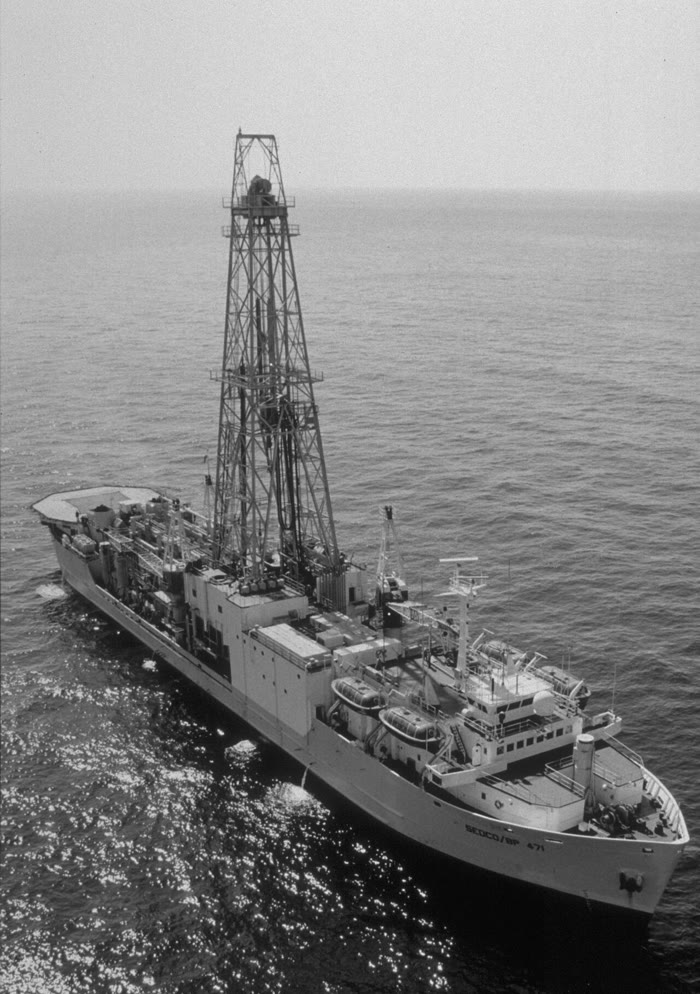
\includegraphics[width=0.36\linewidth]{images/book2/g11-odp-joides-resolution.jpg}

{\small वेधन-जहाज़ \emph{जॉइडीज़ रेज़ोल्यूशन}, जो
\emph{ग्लोमार चैलेंजर} का उत्तराधिकारी बना: ऊँचा मीनार इसका वेधन-डेरिक है, और
जहाज़ \qty{9000}{m} से अधिक वेधन-नली ले जाता है। फ़ोटो: महासागर वेधन कार्यक्रम, टेक्सस A\&M
विश्वविद्यालय (सार्वजनिक डोमेन)।}
\end{omfigure}
% ledger: photo:g11-joides, usgs:glomar

तब से हज़ारों चुंबकीय प्रोफ़ाइलें और सैकड़ों वेधन-छिद्र मिलाकर
पूरी महासागरीय तली की आयु का मानचित्र बनाया गया है।

\begin{omfigure}
\begin{tikzpicture}
\begin{axis}[ommap, width=\linewidth, xtick=\empty, ytick=\empty, grid=none,
    axis background/.style={}, clip=true, name=map]
  \addplot graphics[xmin=-180, xmax=180, ymin=-90, ymax=90] {figdata/out/grade-11-seafloor_age.png};
  \addplot[black!60, line width=0.15pt] table {figdata/out/shared-geo-land.dat};
\end{axis}
\begin{axis}[at={(map.south)}, anchor=north, yshift=-0.35cm, scale only axis, width=0.55\linewidth, height=0.32cm,
    xmin=0, xmax=200, ymin=0, ymax=1, axis y line=none, axis x line*=bottom,
    xtick={0,20,...,180}, tick label style={font=\scriptsize},
    xlabel={महासागरीय तली की आयु (मिलियन वर्ष); धूसर: कोई महासागरीय तली नहीं}, label style={font=\scriptsize},
    enlargelimits=false]
  \addplot graphics[xmin=0, xmax=200, ymin=0, ymax=1] {figdata/out/grade-11-seafloor_age-bar.png};
\end{axis}
\end{tikzpicture}

{\small महासागरीय तली की आयु। कटकों के अनुदिश सबसे नई (लाल), यह उनसे दोनों ओर दूर
जाने पर पुरानी होती जाती है; सबसे पुरानी तली (नीली और बैंगनी)
महासागरों के किनारों पर, महाद्वीपों से सटकर और खाइयों के अनुदिश है।
आँकड़े: सेटन और अन्य (2020), 1-अंश के कोष्ठों में; स्थल की रूपरेखाएँ: नैचुरल
अर्थ।}
\end{omfigure}
% ledger: data:b2-seafloor-age, data:ne-land (map computed in figdata/grade-11/seafloor_age.py)

मानचित्र एक साथ हर बात की पुष्टि करता है। हर कटक के अनुदिश तली नई है,
और उसकी आयु उससे दूर सममित रूप से बढ़ती है। कोई महासागरीय तली
लगभग \num{190} मिलियन वर्ष से अधिक पुरानी नहीं है: सबसे पुरानी पश्चिमी प्रशांत में और
उत्तरी अमेरिका के पूर्वी तट के पास है (पूर्वी भूमध्य सागर की कुछ छोटी द्रोणियाँ
अलग गिनी जाती हैं)। महासागरीय तली की माध्य आयु लगभग
\num{64} मिलियन वर्ष है, और उसका लगभग तीन-चौथाई भाग 100
मिलियन वर्ष से कम पुराना है --- जबकि महाद्वीप कहीं अधिक पुरानी चट्टानें रखते हैं।
महासागरीय तली इसलिए नई है कि वह कटकों पर लगातार बनती रहती है और, जैसा
हेस ने देखा, कहीं और नष्ट होती है: कहाँ, यह
\cref{ch:g11:subduction-zones} का विषय है।
% ledger: data:b2-seafloor-age (oldest_open_myr 192.5, share_younger_100 0.76 in figdata/grade-11/seafloor_age.py), seton:mean-age, usgs:hess

\section{अभ्यास}

\begin{exercise}[$\star$]\label{exo:g11:drift-to-spreading:1}
\omterm{def:g11:drift-to-spreading:spreading}{समुद्री तल प्रसरण} की परिभाषा दीजिए। किसी कटक की पूर्ण और
अर्ध \omterm{def:g11:drift-to-spreading:spreading-rate}{प्रसरण दर} में क्या अंतर है?
\end{exercise}

\begin{exercise}[$\star$]\label{exo:g11:drift-to-spreading:2}
लावा पृथ्वी के क्षेत्र की दिशा केवल लगभग \qty{580}{\celsius} से नीचे ठंडा हो जाने के बाद ही
क्यों अंकित करता है? यदि चट्टान को बाद में \qty{700}{\celsius} तक गरम किया जाए
तो उस अभिलेख का क्या होता है?
\end{exercise}

\begin{exercise}[$\star$]\label{exo:g11:drift-to-spreading:3}
एक प्रतिध्वनि-गहराईमापी अपना स्पंद भेजने के \qty{5.2}{s} बाद उसकी प्रतिध्वनि सुनता है।
समुद्री जल में ध्वनि की चाल \qty{1500}{m/s} लेकर बताइए कि समुद्री तल
कितना गहरा है।
\end{exercise}

\begin{exercise}[$\star$]\label{exo:g11:drift-to-spreading:4}
इस अध्याय के ध्रुवता काल-मापक्रम पर: वर्तमान सामान्य
अंतराल कितने समय से चल रहा है? हारामियो घटना कितने समय चली? पिछले पाँच मिलियन वर्षों में
कितने उत्क्रमण हुए?
\end{exercise}

\begin{exercise}[$\star$]\label{exo:g11:drift-to-spreading:5}
मध्य-महासागरीय कटक लगभग \qty{65000}{km} लंबे हैं। पृथ्वी की परिधि
लगभग \qty{40000}{km} है। कटक पृथ्वी के चारों ओर कितनी बार
लिपट जाते?
\end{exercise}

\begin{exercise}[$\star\star$]\label{exo:g11:drift-to-spreading:6}
किसी चुंबकीय प्रोफ़ाइल पर ब्रून और मातुयामा अंतरालों के बीच की सीमा
(\num{0.78} मिलियन वर्ष) कटक-अक्ष से \qty{20}{km} पर है। अर्ध दर और पूर्ण दर
सेंटीमीटर प्रति वर्ष में परिकलित कीजिए।
\end{exercise}

\begin{exercise}[$\star\star$]\label{exo:g11:drift-to-spreading:7}
एक और प्रोफ़ाइल पर गाउस--गिल्बर्ट सीमा (\num{3.58} मिलियन वर्ष)
अक्ष से \qty{45}{km} पश्चिम और \qty{44}{km} पूर्व में है। हर ओर अर्ध दर
और पूर्ण दर परिकलित कीजिए। क्या प्रसरण सममित है?
\end{exercise}

\begin{exercise}[$\star\star$]\label{exo:g11:drift-to-spreading:8}
1968 के वेधन का स्थल 19 मध्य-अटलांटिक कटक के अक्ष से \qty{990}{km} पर
है। प्रति वर्ष \qty{1.9}{cm} की अर्ध दर से वहाँ की तली की आयु का पूर्वानुमान
लगाइए, और उसकी तुलना उसके सबसे पुराने अवसाद के \num{49} मिलियन वर्षों से
कीजिए।
\end{exercise}

\begin{exercise}[$\star\star$]\label{exo:g11:drift-to-spreading:9}
एक कटक प्रति वर्ष \qty{2}{cm} की अर्ध दर से फैलता है। इस अध्याय के काल-मापक्रम की
सहायता से 0.78,
0.99, 1.07, 1.77 और 1.95 मिलियन वर्ष की सीमाओं की अक्ष से दूरियाँ बताइए, और एक ओर की धारियाँ बनाइए,
सामान्य को काले रंग में।
\end{exercise}

\begin{exercise}[$\star\star$]\label{exo:g11:drift-to-spreading:10}
महासागरीय तली की माध्य आयु लगभग \num{64} मिलियन वर्ष है; पृथ्वी
लगभग \num{4.6} अरब वर्ष पुरानी है। यह पृथ्वी की आयु का कितना अंश है?
यह हेस के किस तर्क का समर्थन करता है?
\end{exercise}

\begin{exercise}[$\star\star$]\label{exo:g11:drift-to-spreading:11}
एक चित्र के साथ समझाइए कि किसी कटक के एक ओर की चुंबकीय धारियों का प्रतिरूप
दूसरी ओर के प्रतिरूप का दर्पण-प्रतिबिंब क्यों है। कौन-सी चीज़
इस सममिति को तोड़ देगी?
\end{exercise}

\begin{exercise}[$\star\star\star$]\label{exo:g11:drift-to-spreading:12}
मान लीजिए कि कुल \qty{65000}{km} लंबे कटक प्रति वर्ष \qty{5}{cm} की औसत पूर्ण दर से
फैलते हैं।
\begin{enumerate}
  \item वे हर वर्ष कितना नया महासागरीय तल क्षेत्रफल बनाते हैं, \unit{km^2} में?
  \item महासागरीय तली लगभग \qty{2.9e8}{km^2} में फैली है। कटकों को
        इतना बनाने में कितना समय लगेगा?
  \item इसकी तुलना सबसे पुरानी महासागरीय तली, लगभग \num{190} मिलियन वर्ष, से कीजिए।
        महासागरीय तली के साथ उतनी ही तेज़ी से क्या होना चाहिए जितनी तेज़ी से वह बनती है?
\end{enumerate}
\end{exercise}

\begin{exercise}[$\star\star\star$]\label{exo:g11:drift-to-spreading:13}
हारामियो घटना \num{0.99} से \num{1.07} मिलियन वर्ष पहले तक चली।
\qty{1.25}{cm} प्रति वर्ष की अर्ध दर वाले कटक के, और \qty{7.5}{cm} प्रति वर्ष वाले कटक के, हर ओर
इसकी धारी कितनी चौड़ी है? चुंबकित
चट्टान समुद्र की सतह से लगभग \qty{3}{km} नीचे है। समझाइए कि यह घटना
इस अध्याय की तेज़ प्रोफ़ाइल पर साफ़ क्यों दिखती है पर धीमी प्रोफ़ाइल पर लगभग नहीं।
\end{exercise}

\begin{exercise}[$\star\star\star$]\label{exo:g11:drift-to-spreading:14}
1968 के स्थलों पर अवसाद स्थल 16 पर \qty{176}{m} मोटा है, जिसकी तली
लगभग \num{11} मिलियन वर्ष पुरानी है, और स्थल 20 पर केवल \qty{72}{m} मोटा,
जो लगभग \num{67} मिलियन वर्ष पुराना है। हर स्थल पर अवसाद के जमा होने की औसत दर
परिकलित कीजिए, मीटर प्रति मिलियन वर्ष में। क्या
अवसाद की मोटाई से तली का काल-निर्धारण किया जा सकता है? इसके बजाय किसका उपयोग होता है?
\end{exercise}

\begin{exercise}[$\star\star\star$]\label{exo:g11:drift-to-spreading:15}
किसी कटक के आर-पार की एक प्रोफ़ाइल पर \num{2.581} मिलियन वर्ष की सीमा
अक्ष से \qty{58}{km} पश्चिम और \qty{70}{km} पूर्व में है।
\begin{enumerate}
  \item हर ओर अर्ध दर और पूर्ण दर परिकलित कीजिए।
  \item अक्ष के पूर्व की तली उसके पश्चिम की तली से अधिक तेज़ी से बनी।
        यदि ये दरें 10 मिलियन वर्ष तक बनी रहें, तो उस आयु, यानी 10 मिलियन
        वर्ष, की तली हर ओर अक्ष से कितनी दूर होगी?
  \item समझाइए कि दोनों सीमाओं के बीच की दूरी पूर्ण
        दर क्यों देती है, भले ही प्रसरण सममित न हो।
\end{enumerate}
\end{exercise}

\section{समस्या: दक्षिण अटलांटिक की आयु}

\begin{problem}[{सप्ताहांत समस्या --- तीन ढंगों से एक महासागर का काल-निर्धारण}]
\label{pb:g11:drift-to-spreading:1}
% ledger: dsdp3:table5, dsdp3:rate, data:b2-seafloor-age, earth:Rmean, ics:base.Cretaceous
% (values computed in figdata/grade-11/sediment_ages.py and seafloor_age.py)
1968 में \emph{ग्लोमार चैलेंजर} ने लगभग \ang{30} दक्षिण अक्षांश के पास
मध्य-अटलांटिक कटक के आर-पार सात छेद किए। तालिका हर
स्थल के लिए कटक-अक्ष से उसकी दूरी, बेसाल्ट पर के सबसे पुराने अवसाद की
आयु (उसके जीवाश्मों से) और, जहाँ उसके नीचे की धारी पहचानी गई, उस
चुंबकीय धारी की आयु देती है, मिलियन वर्षों में।

\begin{center}
\small
\begin{tabular}{|c|c|c|c|}
\hline
स्थल & अक्ष से दूरी (\unit{km}) & सबसे पुराने अवसाद की आयु & चुंबकीय धारी की आयु \\ \hline
16 & 191 & 11 & 9 \\ \hline
15 & 380 & 24 & 21 \\ \hline
18 & 506 & 26 & --- \\ \hline
17 & 643 & 33 & --- \\ \hline
14 & 727 & 40 & 38.5 \\ \hline
19 & 990 & 49 & 53 \\ \hline
20 & 1270 & 67 & 71 \\ \hline
\end{tabular}

{\small आँकड़े: गहन समुद्र वेधन परियोजना, चरण 3 (1970); चुंबकीय आयु वहाँ दिए गए परिसरों
के मध्य-बिंदु हैं।}
\end{center}

\begin{center}
\begin{tikzpicture}
\begin{axis}[omrecord, width=0.82\linewidth, height=5.0cm, xmin=-50, xmax=16, ymin=0, ymax=140,
  xlabel={\ang{30} दक्षिण के अनुदिश देशांतर (अंश; ऋणात्मक: पश्चिम)}, ylabel={आयु (मिलियन वर्ष)},
  tick label style={font=\small}, label style={font=\small}, clip=false]
\addplot[omDef, line width=0.8pt] table[x=lon, y=age] {figdata/out/grade-11-seafloor_age-profile.dat};
\draw[omRidge, densely dashed] (axis cs:-13.8,0) -- (axis cs:-13.8,140);
\node[font=\scriptsize, text=omRidge, anchor=south] at (axis cs:-13.8,140) {कटक-अक्ष};
\fill (axis cs:-47.4,125.1) circle (1.5pt);
\node[font=\scriptsize, anchor=south west, inner sep=2pt] at (axis cs:-47.6,126) {दक्षिण अमेरिका};
\node[font=\scriptsize, anchor=north west, align=left] at (axis cs:14.2,135) {अफ़्रीका};
\fill (axis cs:13.8,129.8) circle (1.5pt);
\end{axis}
\end{tikzpicture}

{\small दक्षिण अमेरिका से अफ़्रीका तक \ang{30} दक्षिण अक्षांश रेखा के अनुदिश महासागरीय तली की
आयु; रेखा वहाँ रुकती है जहाँ महासागरीय तली हर
महाद्वीप से सटकर समाप्त होती है। आँकड़े: सेटन और अन्य (2020)।}
\end{center}

\medskip
\noindent\textbf{भाग I --- वेधन-स्थल।}
\begin{enumerate}
  \item कौन-सा स्थल कटक के सबसे निकट है, और कौन-सा सबसे दूर? उनकी
        आयुओं की तुलना कैसी है?
  \item बेसाल्ट पर पड़े सबसे पुराने अवसाद की आयु स्वयं बेसाल्ट की आयु के
        निकट क्यों है? क्या वह थोड़ी अधिक है या थोड़ी
        कम?
  \item हर स्थल के लिए उसकी दूरी और उसके सबसे पुराने अवसाद की आयु का अनुपात,
        किलोमीटर प्रति मिलियन वर्ष में, परिकलित कीजिए।
  \item इन सात अनुपातों का माध्य क्या है? इसे सेंटीमीटर प्रति
        वर्ष में बदलिए।
  \item स्थल 17 और 18 कटक के पूर्व में हैं, बाक़ी पश्चिम में। क्या
        पूर्वी स्थल पश्चिमी स्थलों की ही प्रवृत्ति का अनुसरण करते हैं? इससे
        प्रसरण के बारे में क्या पता चलता है?
\end{enumerate}

\medskip
\noindent\textbf{भाग II --- अवसादों से दर।}
\begin{enumerate}[resume]
  \item यदि तली नियत अर्ध दर $u$ से फैली होती, तो तली की आयु
        $t$ अक्ष से उसकी दूरी $d$ पर कैसे निर्भर करती?
  \item मूल-बिंदु से होकर जाने वाली वह रेखा जो बिंदुओं से सबसे अच्छा मेल खाती है, उसकी ढाल
        $u = \sum d\,t / \sum t^2$ है। सात स्थलों के लिए
        $\sum d\,t = \num{208276}$ और $\sum t^2 = \num{10952}$ (किलोमीटर
        और मिलियन वर्षों में)। $u$ को किलोमीटर प्रति
        मिलियन वर्ष में और सेंटीमीटर प्रति वर्ष में परिकलित कीजिए।
  \item इस अक्षांश पर दक्षिण अटलांटिक की \omterm{def:g11:drift-to-spreading:spreading-rate}{पूर्ण प्रसरण दर} क्या है?
  \item अभियान के वैज्ञानिकों ने लिखा कि दर ``प्रति वर्ष \qty{2}{cm} से
        थोड़ी कम'' थी। क्या आप सहमत हैं?
  \item इस दर से स्थल 20 पर तली की आयु का पूर्वानुमान लगाइए, और उसकी तुलना
        उसके सबसे पुराने अवसाद से कीजिए।
\end{enumerate}

\medskip
\noindent\textbf{भाग III --- चुंबकीय धारियों से दर।}
\begin{enumerate}[resume]
  \item केवल स्थल 16 से (\qty{191}{km}, 9 मिलियन वर्ष की धारी)
        एक अर्ध दर परिकलित कीजिए।
  \item केवल स्थल 20 से (\qty{1270}{km}, 71 मिलियन वर्ष की धारी)
        एक अर्ध दर परिकलित कीजिए।
  \item चुंबकीय आयु वाले पाँच स्थलों के लिए $\sum d\,t = \num{180329}$ और
        $\sum t^2 = \num{9854}$। सबसे अच्छी अर्ध दर परिकलित कीजिए।
  \item जीवाश्मों से और धारियों से मिली दरों में कितने प्रतिशत का
        अंतर है? क्या दोनों विधियाँ सहमत हैं?
  \item यह क्यों महत्त्वपूर्ण है कि दोनों आयु बिल्कुल
        अलग-अलग विधियों से निकाली गईं?
\end{enumerate}

\medskip
\noindent\textbf{भाग IV --- महासागर के किनारे तक।}
\begin{enumerate}[resume]
  \item \ang{30} दक्षिण के अनुदिश कटक-अक्ष देशांतर
        \ang{13.8} पश्चिम पर है और महासागरीय तली अफ़्रीका से सटकर
        \ang{13.8} पूर्व पर समाप्त होती है। उन्हें देशांतर के कितने अंश अलग करते हैं?
  \item \qty{6371}{km} त्रिज्या के गोले पर देशांतर का एक अंश
        $\qty{111.2}{km} \times \cos(\text{अक्षांश})$ मापता है। \ang{30} दक्षिण पर एक अंश की
        लंबाई परिकलित कीजिए, और अक्ष से अफ़्रीका के पास महासागरीय तली के किनारे तक की
        दूरी।
  \item यदि तली हमेशा भाग II की दर से फैली होती, तो किनारे की तली कितने
        समय पहले बनी होती?
  \item आयु-मानचित्र, जो पुरानी तली का काल-निर्धारण उसकी चुंबकीय धारियों से करता है, किनारे पर
        \num{130} मिलियन वर्ष देता है। इससे कौन-सी औसत अर्ध दर
        निकलती है? क्या महासागर का आरंभिक खुलना पिछले 66 मिलियन वर्षों के खुलने से
        थोड़ा तेज़ था या थोड़ा धीमा?
  \item निष्कर्ष निकालिए: \ang{30} दक्षिण पर अफ़्रीका के पास की सबसे पुरानी महासागरीय तली
        कितनी पुरानी है? क्रिटेशस कल्प लगभग \num{143} मिलियन
        वर्ष पहले शुरू हुआ: दक्षिण अटलांटिक वहाँ किस कल्प में खुलना
        शुरू हुआ?
\end{enumerate}
\end{problem}
